\section*{Indtegning af den rette linje i koordinatsystemet}

For at indtegne en ret linje i et koordinatsystem kan vi benytte os af sildeben. Et sildeben ser typsisk sådan ud

\begin{tabular}{c|c|c|c|c}
x & -1 & 0 & 1 & 2 \\\hline
y &  & &   &  
\end{tabular}

Her vælger vi typisk x værdier omkring værdien 0. Vi bruger så den rette linjes forskrift til at bestemme de tilsvarende y værdier. For hver kolonne i sildebenet har vi altså nogle punkter som den rette linje går igennem. Indtegner vi punkterne i koordinatsystemet og forbinder dem med en ret linje har vi dermed indtegnet en ret linje i koordinatsystemet.

\subsection*{Eksempel 1:}

Indtegn den rette linje med forskriften $y = 2x - 1$ i koordinatsystemet.

Vi bruger sildebenet \begin{tabular}{c|c|c|c|c}
x & -1 & 0 & 1 & 2 \\\hline
y &  & &   &  
\end{tabular}

og bestemmer nu de tilsvarende y værdier, ved at indsætte x værdierne på x's plads i forskriften for den rette linje

\begin{align*}
y &= 2\cdot (-1) -1 = -2 -1 = -3 && x = -1\\
y &= 2 \cdot 0 - 1 = 0 - 1 = -1 && x = 0\\
y &= 2 \cdot 1 - 1 = 2 - 1 = 1 && x = 1\\
y &= 2 \cdot 2 - 1 = 4 - 1 = 3 && x = 3
\end{align*}

Vi har nu følgende sildeben

\begin{tabular}{c|c|c|c|c}
x & -1 & 0 & 1 & 2 \\\hline
y & -3 & -1 & 1 & 3 
\end{tabular}

Vi indsætter nu punkterne $(-1, -3), (0, -1), (1, 1), (2, 3)$ i koordinatsystemet og forbinder punkterne med en ret linje som kan ses nedenfor

\begin{figure*}[ht]
    \centering
    \begin{subfigure}[t]{0.5\textwidth}
        \centering
        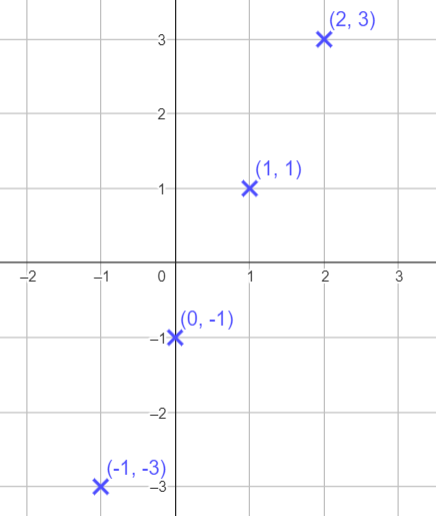
\includegraphics[width=0.5\textwidth]{img_1}
        \caption{Koordinatsystem med punkterne indtegnet}
    \end{subfigure}%
    ~ 
    \begin{subfigure}[t]{0.5\textwidth}
        \centering
        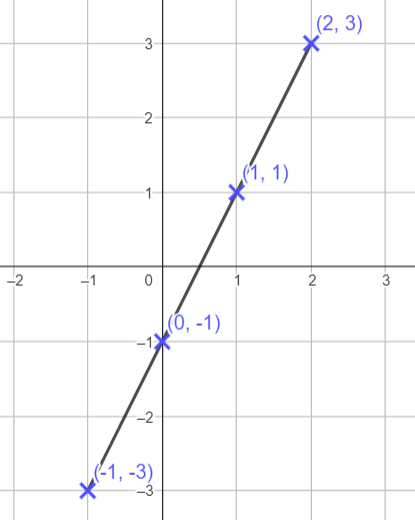
\includegraphics[width=0.5\textwidth]{img_2}
        \caption{Koordinatsystem hvor punkterne er forbundet med en ret linje}
    \end{subfigure}
    \caption{Indtegning af den rette linje $y = 2x - 1$ i koordinatsystemet}
\end{figure*}


\subsection*{Opgaver}


\textbf{Opgave 1:}

Indtegn den rette linje med forskriften $y = -2x - 1$ i koordinatsystemet

\textbf{Opgave 2:}

Indtegn den rette linje med forskriften $y = 3x + 4$ i koordinatsystemet

\textbf{Opgave 3:}

Indtegn den rette linje med forskriften $y = -4x -4$ i koordinatsystemet

\textbf{Opgave 4:}

Indtegn den rette linje med forskriften $y = -5x + 3$ i koordinatsystemet

\textbf{Opgave 5:}

Indtegn den rette linje med forskriften $y = 2x + 6$ i koordinatsystemet





\newpage

\subsection*{Facit}

\textbf{Opgave 1:}

\begin{figure*}[ht]
    \centering
    \begin{subfigure}[t]{0.5\textwidth}
        \centering
        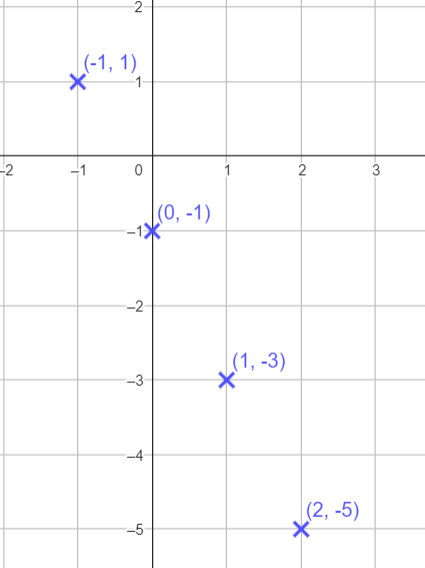
\includegraphics[width=0.5\textwidth]{img_3}
        \caption{Koordinatsystem med punkterne indtegnet}
    \end{subfigure}%
    ~ 
    \begin{subfigure}[t]{0.5\textwidth}
        \centering
        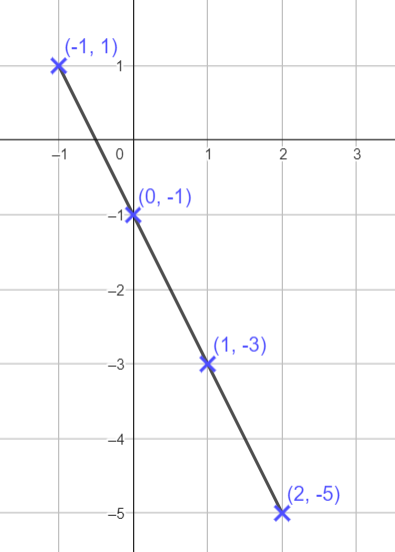
\includegraphics[width=0.5\textwidth]{img_4}
        \caption{Koordinatsystem hvor punkterne er forbundet med en ret linje}
    \end{subfigure}
    \caption{Indtegning af den rette linje $y = -2x -1 $ i koordinatsystemet}
\end{figure*}

\textbf{Opgave 2:}

\begin{figure*}[ht]
    \centering
    \begin{subfigure}[t]{0.5\textwidth}
        \centering
        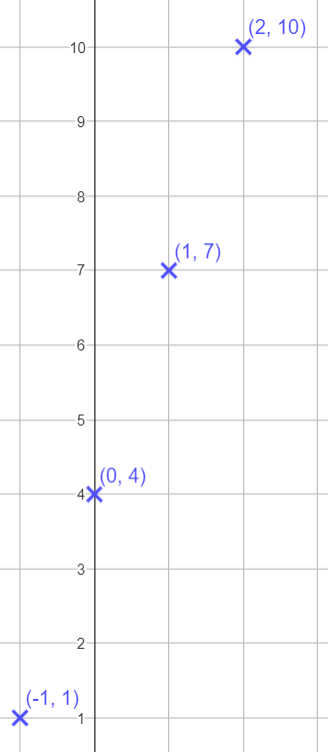
\includegraphics[width=0.5\textwidth, height=0.8\textwidth]{img_5}
        \caption{Koordinatsystem med punkterne indtegnet}
    \end{subfigure}%
    ~ 
    \begin{subfigure}[t]{0.5\textwidth}
        \centering
        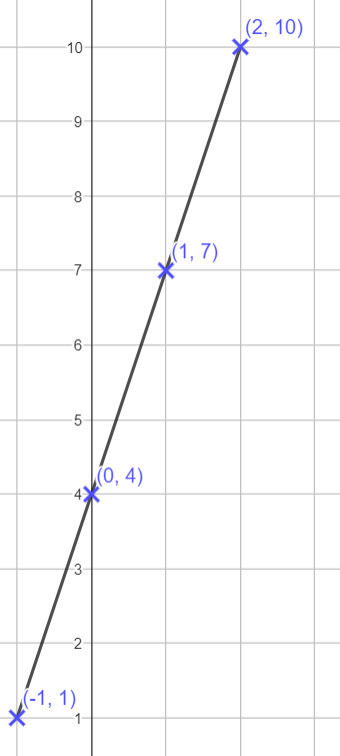
\includegraphics[width=0.5\textwidth, height=0.8\textwidth]{img_6}
        \caption{Koordinatsystem hvor punkterne er forbundet med en ret linje}
    \end{subfigure}
    \caption{Indtegning af den rette linje $y =3x + 4 $ i koordinatsystemet}
\end{figure*}

\newpage

\textbf{Opgave 3:}

\begin{figure*}[ht]
    \centering
    \begin{subfigure}[t]{0.5\textwidth}
        \centering
        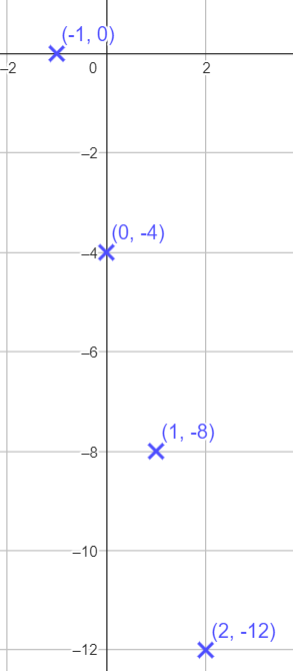
\includegraphics[width=0.5\textwidth, height=0.8\textwidth]{img_7}
        \caption{Koordinatsystem med punkterne indtegnet}
    \end{subfigure}%
    ~ 
    \begin{subfigure}[t]{0.5\textwidth}
        \centering
        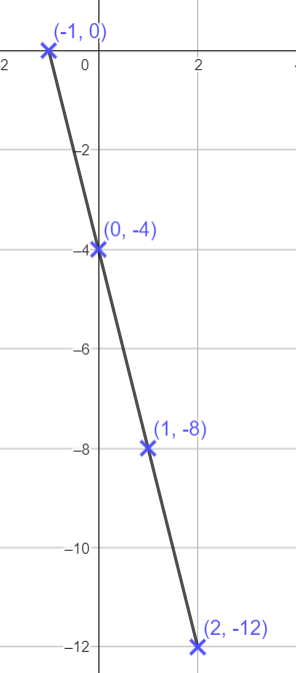
\includegraphics[width=0.5\textwidth, height=0.8\textwidth]{img_8}
        \caption{Koordinatsystem hvor punkterne er forbundet med en ret linje}
    \end{subfigure}
    \caption{Indtegning af den rette linje $y =-4x - 4 $ i koordinatsystemet}
\end{figure*}

\textbf{Opgave 4:}

\begin{figure*}[ht]
    \centering
    \begin{subfigure}[t]{0.5\textwidth}
        \centering
        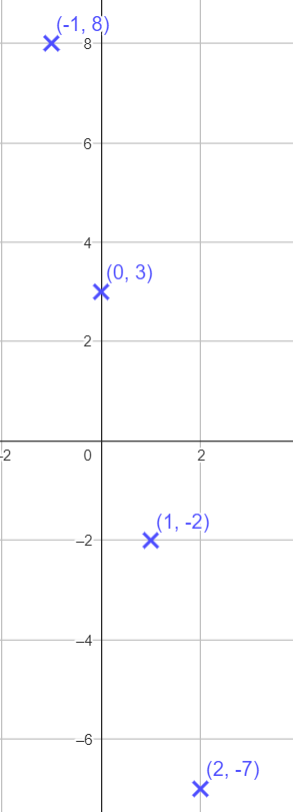
\includegraphics[width=0.5\textwidth, height=0.7\textwidth]{img_9}
        \caption{Koordinatsystem med punkterne indtegnet}
    \end{subfigure}%
    ~ 
    \begin{subfigure}[t]{0.5\textwidth}
        \centering
        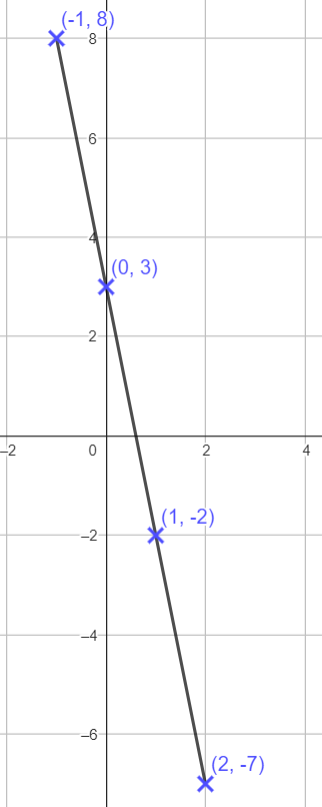
\includegraphics[width=0.5\textwidth, height=0.7\textwidth]{img_10}
        \caption{Koordinatsystem hvor punkterne er forbundet med en ret linje}
    \end{subfigure}
    \caption{Indtegning af den rette linje $y = -5x + 3 $ i koordinatsystemet}
\end{figure*}

\newpage

\textbf{Opgave 5:}

\begin{figure*}[ht]
    \centering
    \begin{subfigure}[t]{0.5\textwidth}
        \centering
        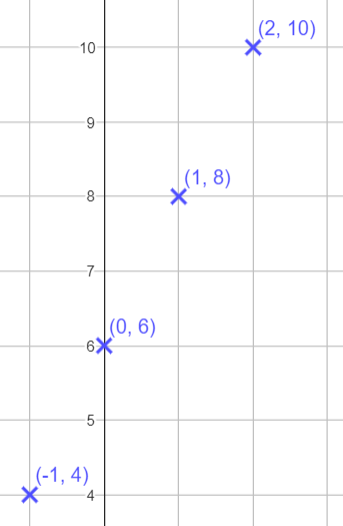
\includegraphics[width=0.5\textwidth, height=0.8\textwidth]{img_11}
        \caption{Koordinatsystem med punkterne indtegnet}
    \end{subfigure}%
    ~ 
    \begin{subfigure}[t]{0.5\textwidth}
        \centering
        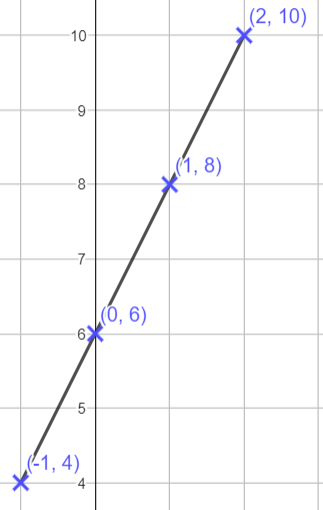
\includegraphics[width=0.5\textwidth, height=0.8\textwidth]{img_12}
        \caption{Koordinatsystem hvor punkterne er forbundet med en ret linje}
    \end{subfigure}
    \caption{Indtegning af den rette linje $y = 2x + 6 $ i koordinatsystemet}
\end{figure*}
